\documentclass{article}
\usepackage[utf8]{inputenc}
\usepackage{graphicx}
\usepackage{float}
\usepackage{geometry}




\geometry{top=3cm, bottom=2cm,left=1cm ,right=1cm}

\begin{document}

\begin{figure}
\centering

\includegraphics[scale=0.1]{logo_TNCY.png}
\label{fig:logo_tncy}
\end{figure}

\title{\bf RAPPORT de Projet}
\author{ Camille COUÉ , Victor COUR , Erwan KESSLER}
\date{\it December 2018}

\maketitle


\title{\bf \Large Sommaire}
\begin{itemize}
    \item Introduction
    \item L'organisation pour répartir le travail 
    \item Gestion des étapes
    \item Production finale : Étape 8
    \item Ce que le projet a apporté à chacun
    \item Remerciements
    \item Sources
    \item État de l'art
\end{itemize}
\section { Introduction }



Le but du projet est de créer un code qui permettrait de choisir la représentation (parmi celles qui sont proposées) où l’on placerait les différents aéroports du monde que le site openflight.org a rescencé en 2017. On pourrait aussi choisir de centrer cette représentation sur une zone souhaitée.

\vspace{1\baselineskip}

Nous avons profité du lendemain de l’annonce du projet pour nous donner rendez-vous dans un restaurant afin de faire connaissance. Après avoir défini l’heure de notre première réunion pour fixer l’organisation du projet , Erwan nous a suggérer de créer un Trello (plateforme de gestion de projet) en attendant que la plateforme Git soit configurée.

\vspace{1\baselineskip}


\section{ L'organisation pour répartir le travail }


Nous avons décidé pour hiérarchiser notre équipe de définir un chef de projet et nous avons convenu que Erwan remplirait ce poste.
Ainsi, Camille et Victor joueront les rôles de secrétaires pour rédiger les comptes rendus à tour de rôle. (Listes des comptes rendus en annexe)

\vspace{1\baselineskip}

La première étape pour se répartir le travail a été de prévoir la durée des tâches, nous avons d’abord effectué un GANTT prévisionnel pour avoir une idée des étapes les plus coûteuse en temps, et à l’inverse, celles qui n’en demandaient pas énormément.

\vspace{1\baselineskip}

\begin{figure}[H]
    \centering
    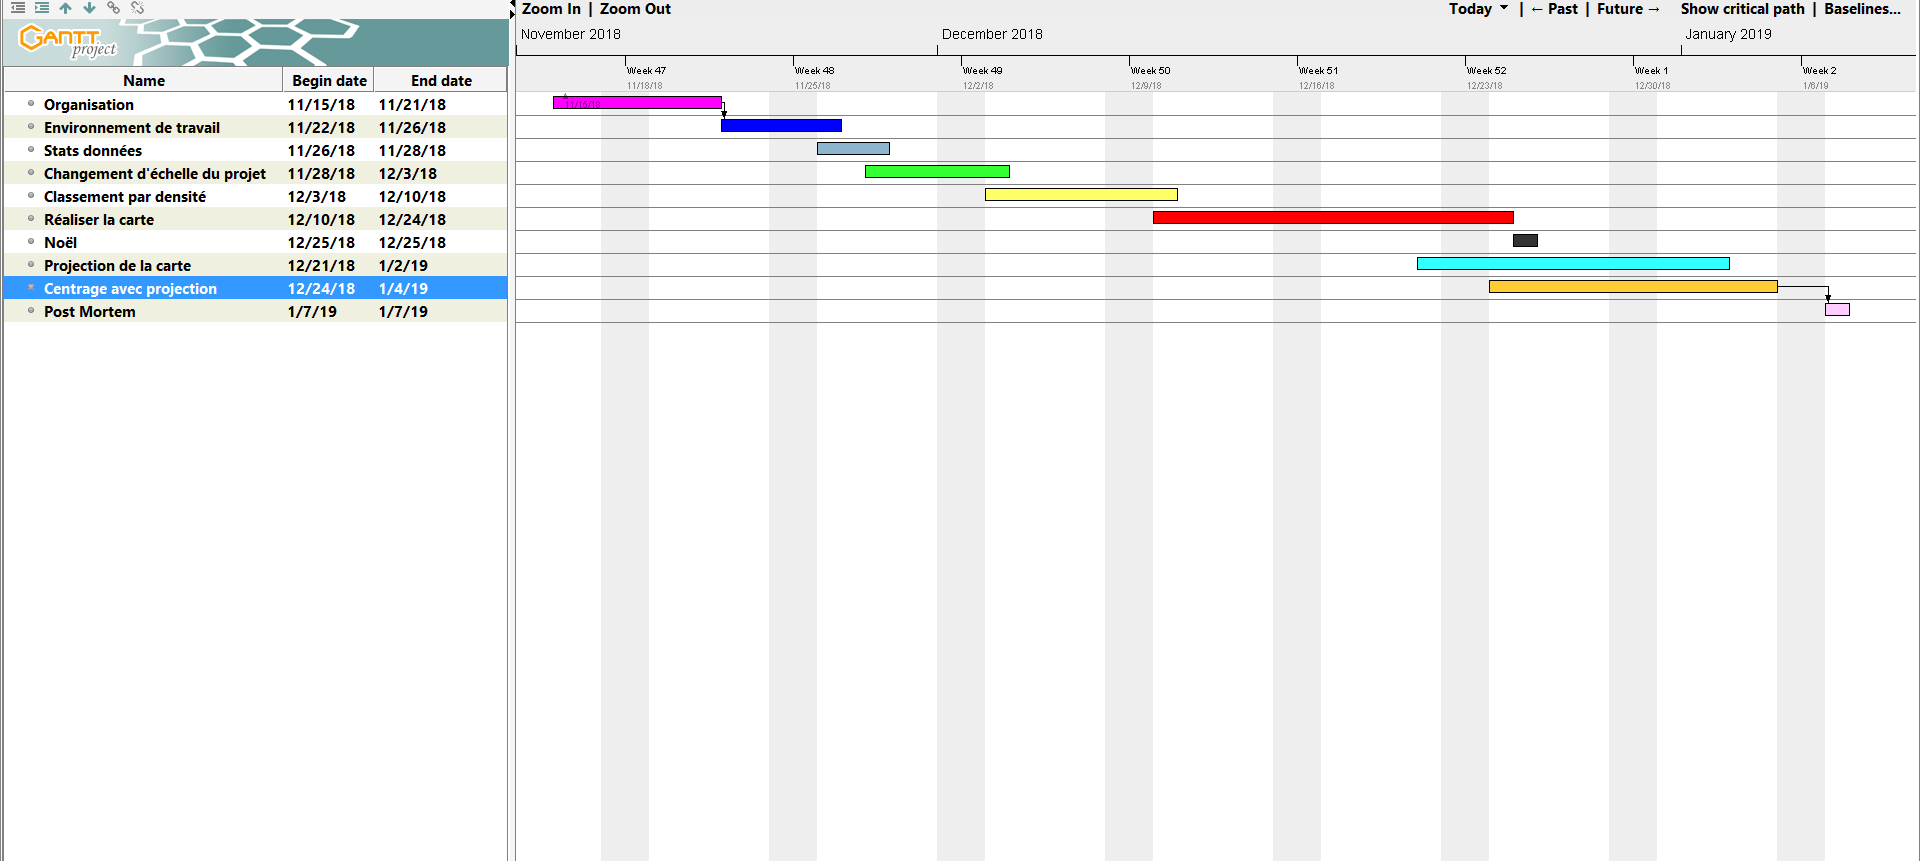
\includegraphics[scale=0.4]{gantt.png}
    \caption{Gantt prévisionnel}
    \label{fig:gantt}
\end{figure}

Nous avons ensuite réparti les tâches avec un responsable pour chacune d’entre elles grâce à une matrice RACI.

\vspace{1\baselineskip}

\begin{figure}[H]
    \centering
    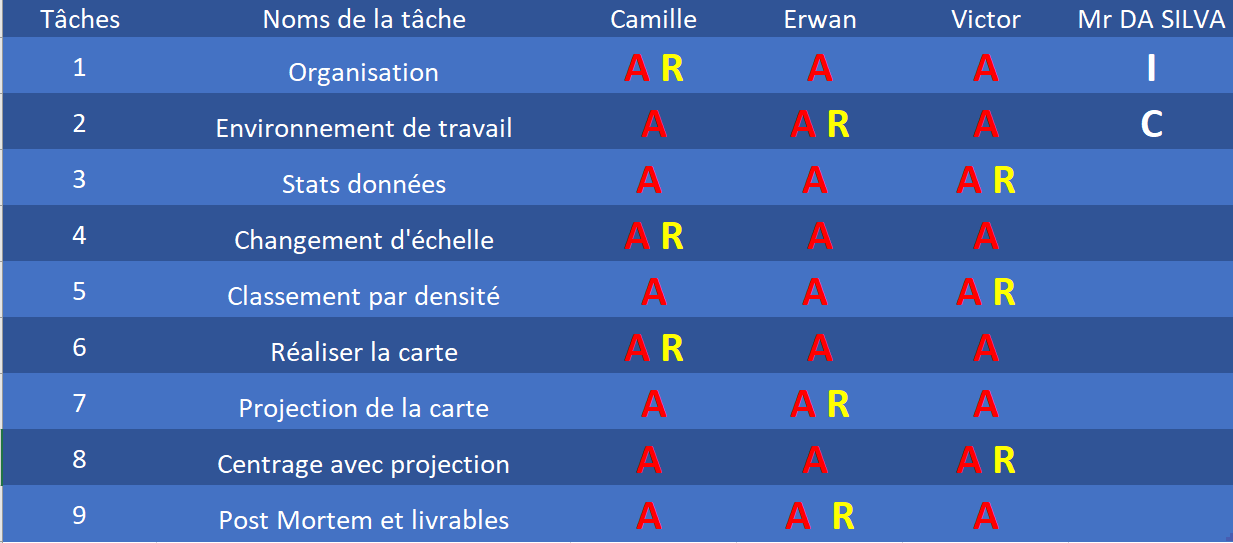
\includegraphics[scale=0.4]{raci.png}
    \caption{Matrice RACI}
    \label{fig:raci}
\end{figure}

\newpage
Enfin, il ne restait plus qu’à prévoir les risques possibles dans le déroulement du projet, c’est pourquoi nous avons utilisé une matrice SWOT pour rendre compte des différents facteurs pouvant nous faire gagner du temps, ou nous en faire perdre.


\begin{figure}[H]
    \centering
    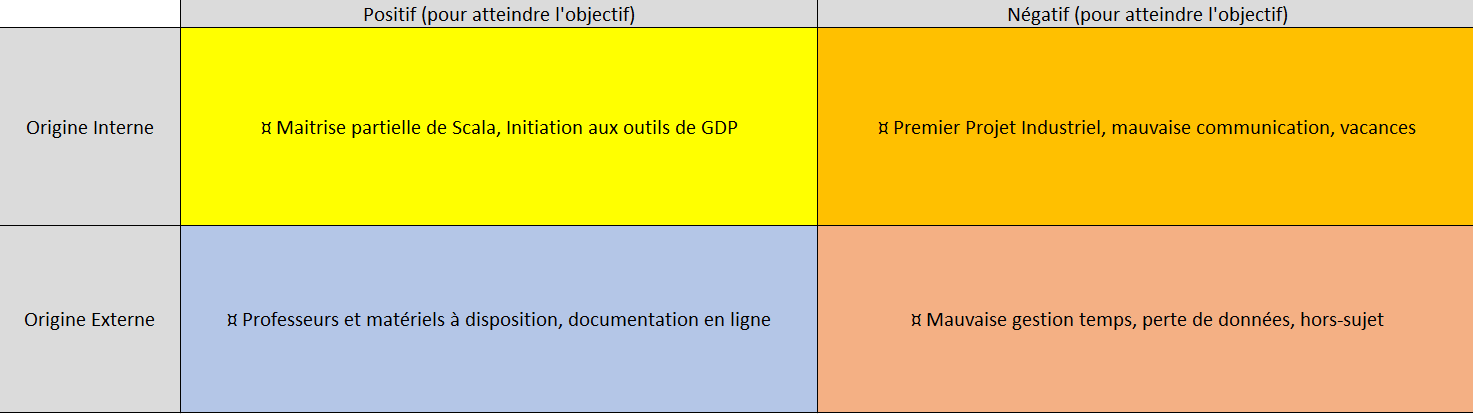
\includegraphics[scale=0.5]{swot.png}
    \caption{Matrice SWOT}
    \label{fig:swot}
\end{figure}

\vspace{3\baselineskip}

\section{ Gestion des étapes}


\subsection{ Étape 1} 


\textbf{Problème rencontré :} \newline
Au premier abord, nous voulions lire le fichier ligne par ligne, et séparer les éléments de ces lignes par des virgules, cependant, il existait des chaînes de caractères possédant des virgules, empêchant la bonne séparation des éléments.

\vspace{1\baselineskip}

\noindent{\textbf{Solution :}} \newline
Suite au problème de séparation des éléments ligne par ligne, il a fallu trouver une expression régulière permettant d’écarter ce problème de virgules en donnant une séparation avec “,” ou “,\textbackslash{} ou encore “,[0-9] qui permettrait de gérer les conflits rencontrés avec les chaînes de caractères possédant des virgules.



\subsection{Étape 2} 


\textbf{Problème rencontré :} \newline
Plusieurs calculs permettant de mesurer une distance existent, l’objectif était de sélectionner la méthode donnant la distance la plus précise possible mais aussi la moins coûteuse en calcul.

\vspace{1\baselineskip}

\noindent{\textbf{Solution :}} \newline
Nous avons alors implémenter plusieurs des méthodes que nous avions trouvées en nous documentant. En testant sur nos données, nous avons remarqué que la méthode d'Harversine était la plus rapide et en plus, la plus précise. Nous avons donc choisi de l'utiliser dans la suite de notre travail. 


\subsection{Étape 3} 


\textbf{Problème rencontré :} \newline
Dans les statistiques, plusieurs méthodes permettaient de calculer la médiane grâce à notre structure de données. Il fallait donc, comme dans l'étape précédante, choisir la "bonne" méthode.

\vspace{1\baselineskip}

\noindent{\textbf{Solution :}} \newline
Ici aussi nous avons selectionné plusieurs méthodes et ensuite testé sur nos données. Nous avons choisi dans un premier temps d'utiliser la fonction .sorted pour trier le tableau, pour ensuite prendre l'élément au milieu (la médiane). Cependant, nous avons cherché pour voir s'il y avait une meilleure méthode que le .sorted, et Erwan a suggeré d'utiliser la méthode du quick select pour trier les données. Il est avéré qu'elle était plus rapide que .sorted.


\subsection{Étape 4} 


Pas de problème particulier sur cette étape.


\subsection{Étape 5}


\textbf{Problème rencontré :} \newline
 Nous avons convenu au départ de compter le nombre d'aéroports dans chaque pays en parcourant notre tableau et en mettant ce résultat dans un autre tableau (avec pour chaque case du tableau un pays lui étant associé). Cependant, il était compliqué d'attribuer un nombre pour chaque pays : la liste des identifiants de "airports.dat" n'étant pas des nombres consécutifs à chaque fois... 
 
\vspace{1\baselineskip}

\noindent{\textbf{Solution :}} \newline
Nous avons décidé d'utiliser les HashMap de la bibliothèque scala.collection.mutable car les HashMap permettent de créer un moyen plus pratique pour accéder aux données que l'on souhaite avoir sous la main. Il faut donc déjà parcourir une fois notre tableau de données pour créer cette HashMap, cependant on accède aux éléments avec une complexité en \textit{O}(1).

\vspace{1\baselineskip}

\subsection{Étape 6} 


\textbf{Problème rencontré :} \newline
L'image wrapper ne fonctionnait pas sur notre version de scala (2.12.7) et les versions supportées étaient "2.9.2", "2.10.6" et "2.11.7".

\vspace{1\baselineskip}

\noindent{\textbf{Solution :}} \newline
Pour régler ce problème de version pour l'image wrapper nous avons décider de regarder sur GitHub pour trouver une version adéquate. [2]


\subsection{Étape 7}


\textbf{Problème rencontré :} \newline
Après s'être documenté sur les projections conformes et équivalentes [1], il fallait transformer un couple (latitude,longitude) en (x,y) avec (x,y) les coordonnées dans la projection voulue. Cependant nous avons remarqué qu'il fallait faire une transformation linéaire sur ces coordonnées pour les placer au bon endroit dans notre image bitmap. Comment trouver ces transformations linéaires?

\vspace{1\baselineskip}
\noindent{\textbf{Solution :}}




 \section{ Production finale : Étape 8}



\newpage

 \section{ Ce que le projet a apporté à chacun}

    Tout d'abord, voici la table des heures que nous avons effectuées.

\begin{figure}[H]
    \centering
    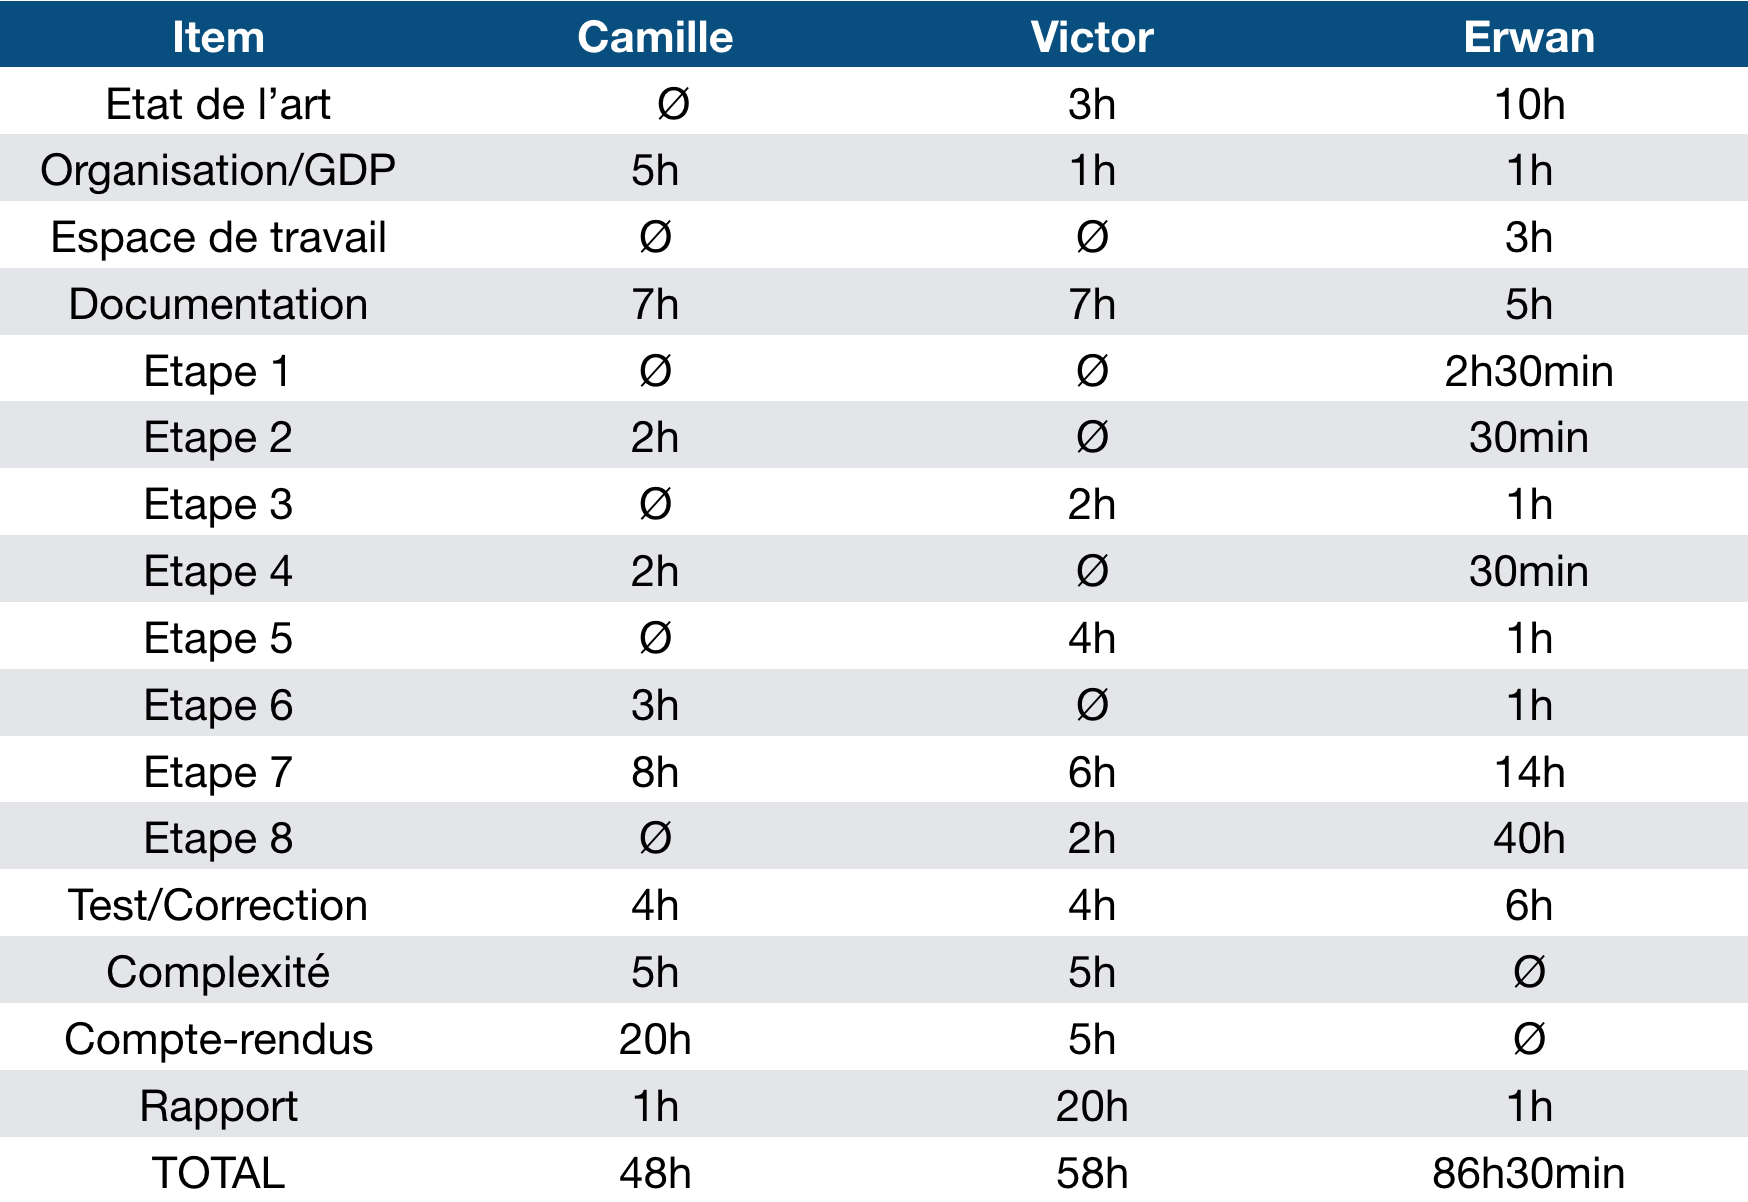
\includegraphics[scale=0.5]{TabledesHeures.png}
    \caption{Table des heures de travail}
    \label{fig:tableheures}
\end{figure}

    Nous avons ensuite fait une réunion post mortem pour évaluer en 2 points ce que le projet nous a apporté : les compétences que nous avons acquises grâce à ce travail, puis les points que nous pensions devoir améliorer.
    
    \newpage
    
    \textbf{Camille :}
    \begin{figure}[H]
        \centering
        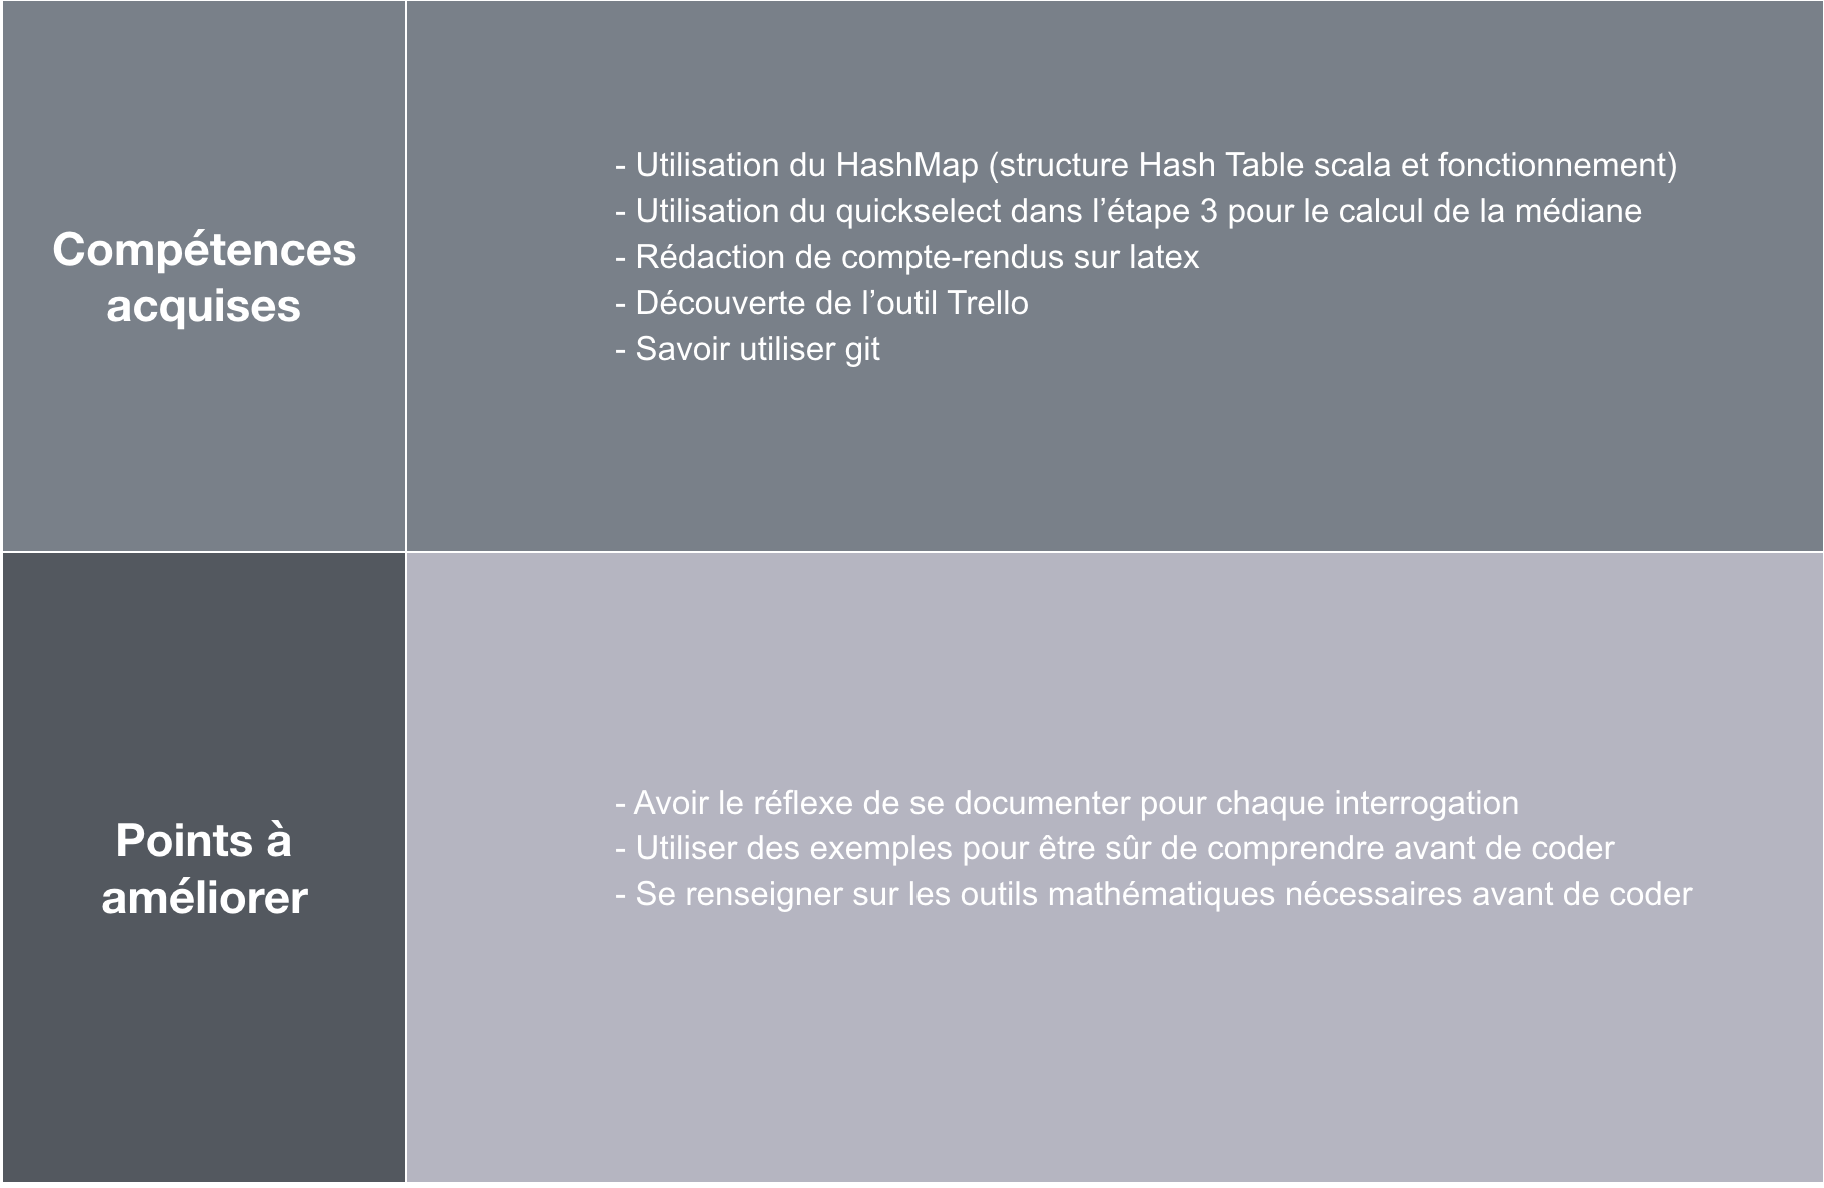
\includegraphics[scale=0.45]{CamillePM.png}
        \caption{CamillePM}
        \label{fig:camillepm}
    \end{figure}
    
    \textbf{Victor :}
    \begin{figure}[H]
        \centering
        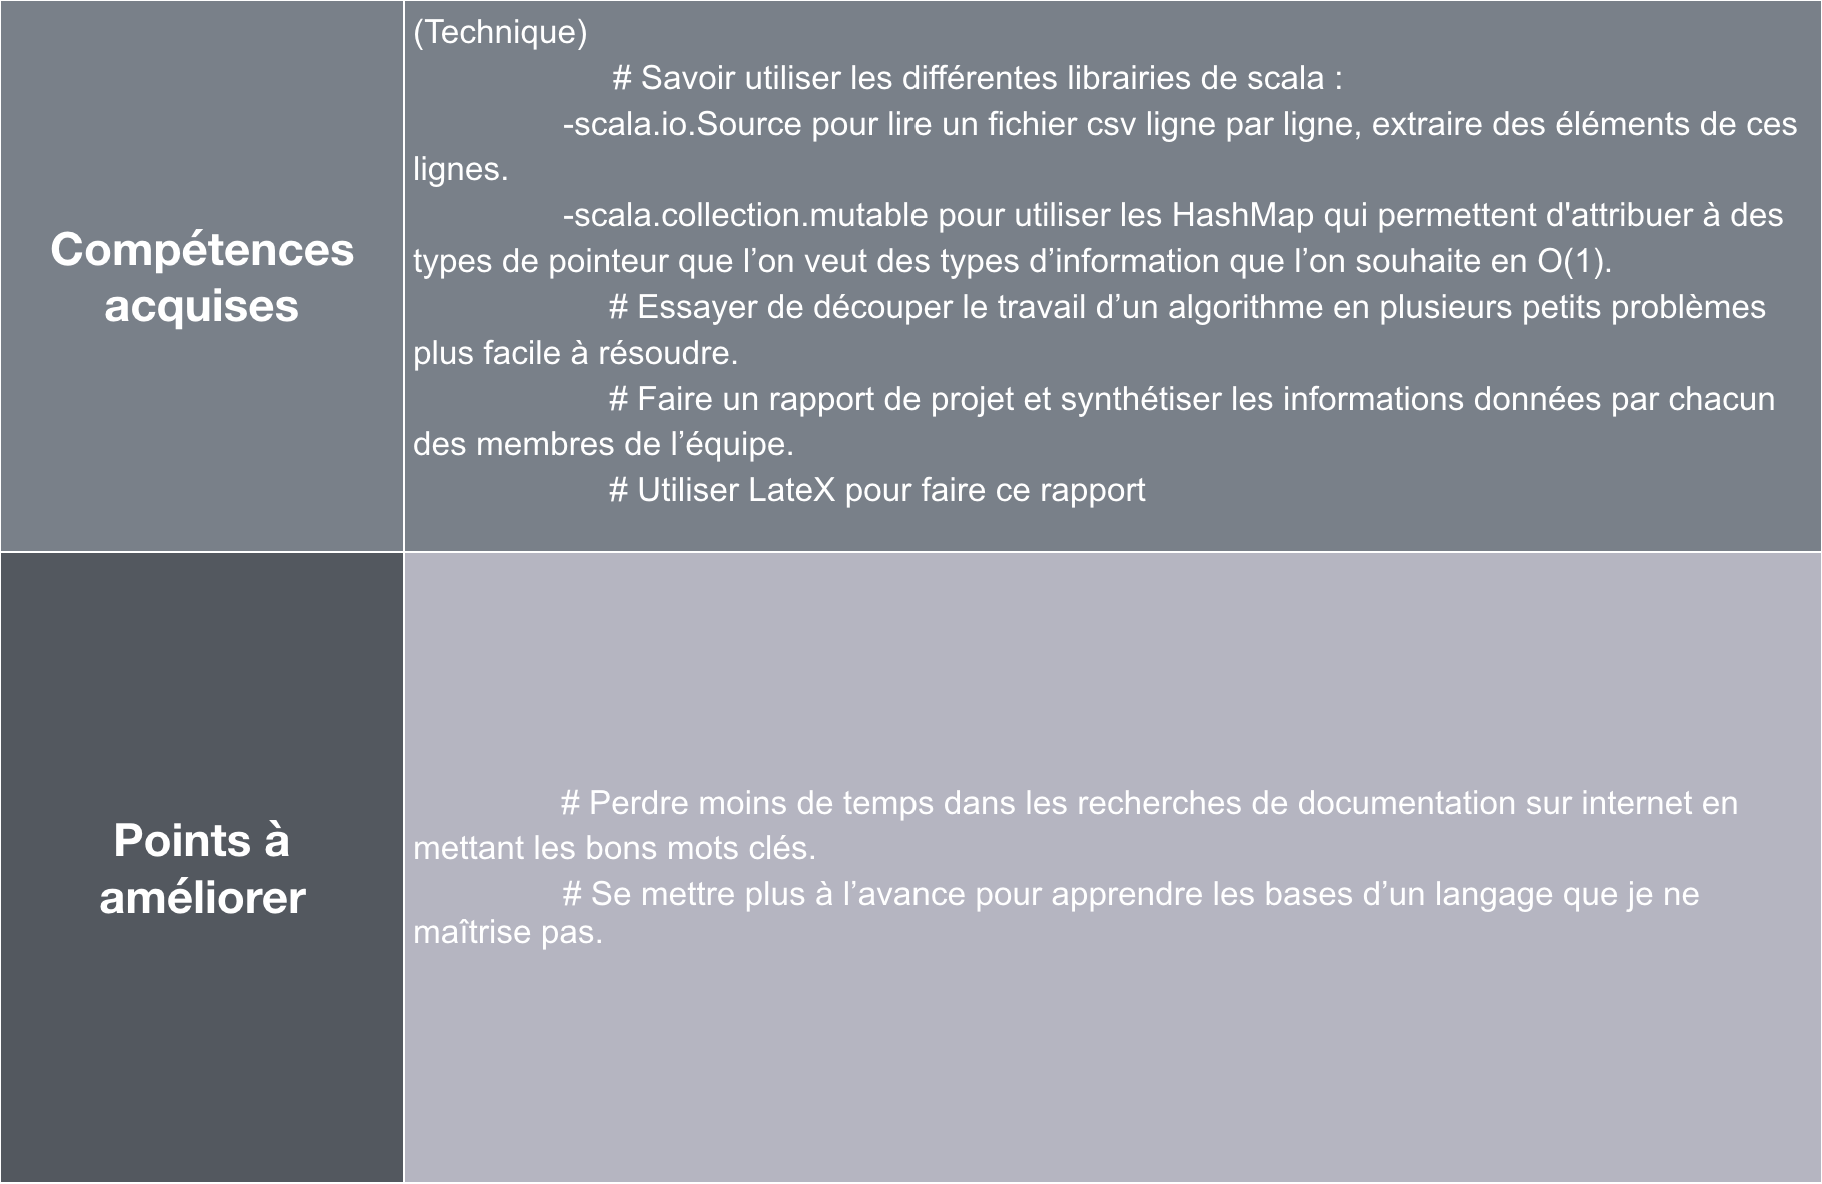
\includegraphics[scale=0.45]{VictorPM.png}
        \caption{VictorPM}
        \label{fig:victorpm}
    \end{figure}
    
    \newpage
    
    \textbf{Erwan :}
    \begin{figure}[H]
        \centering
        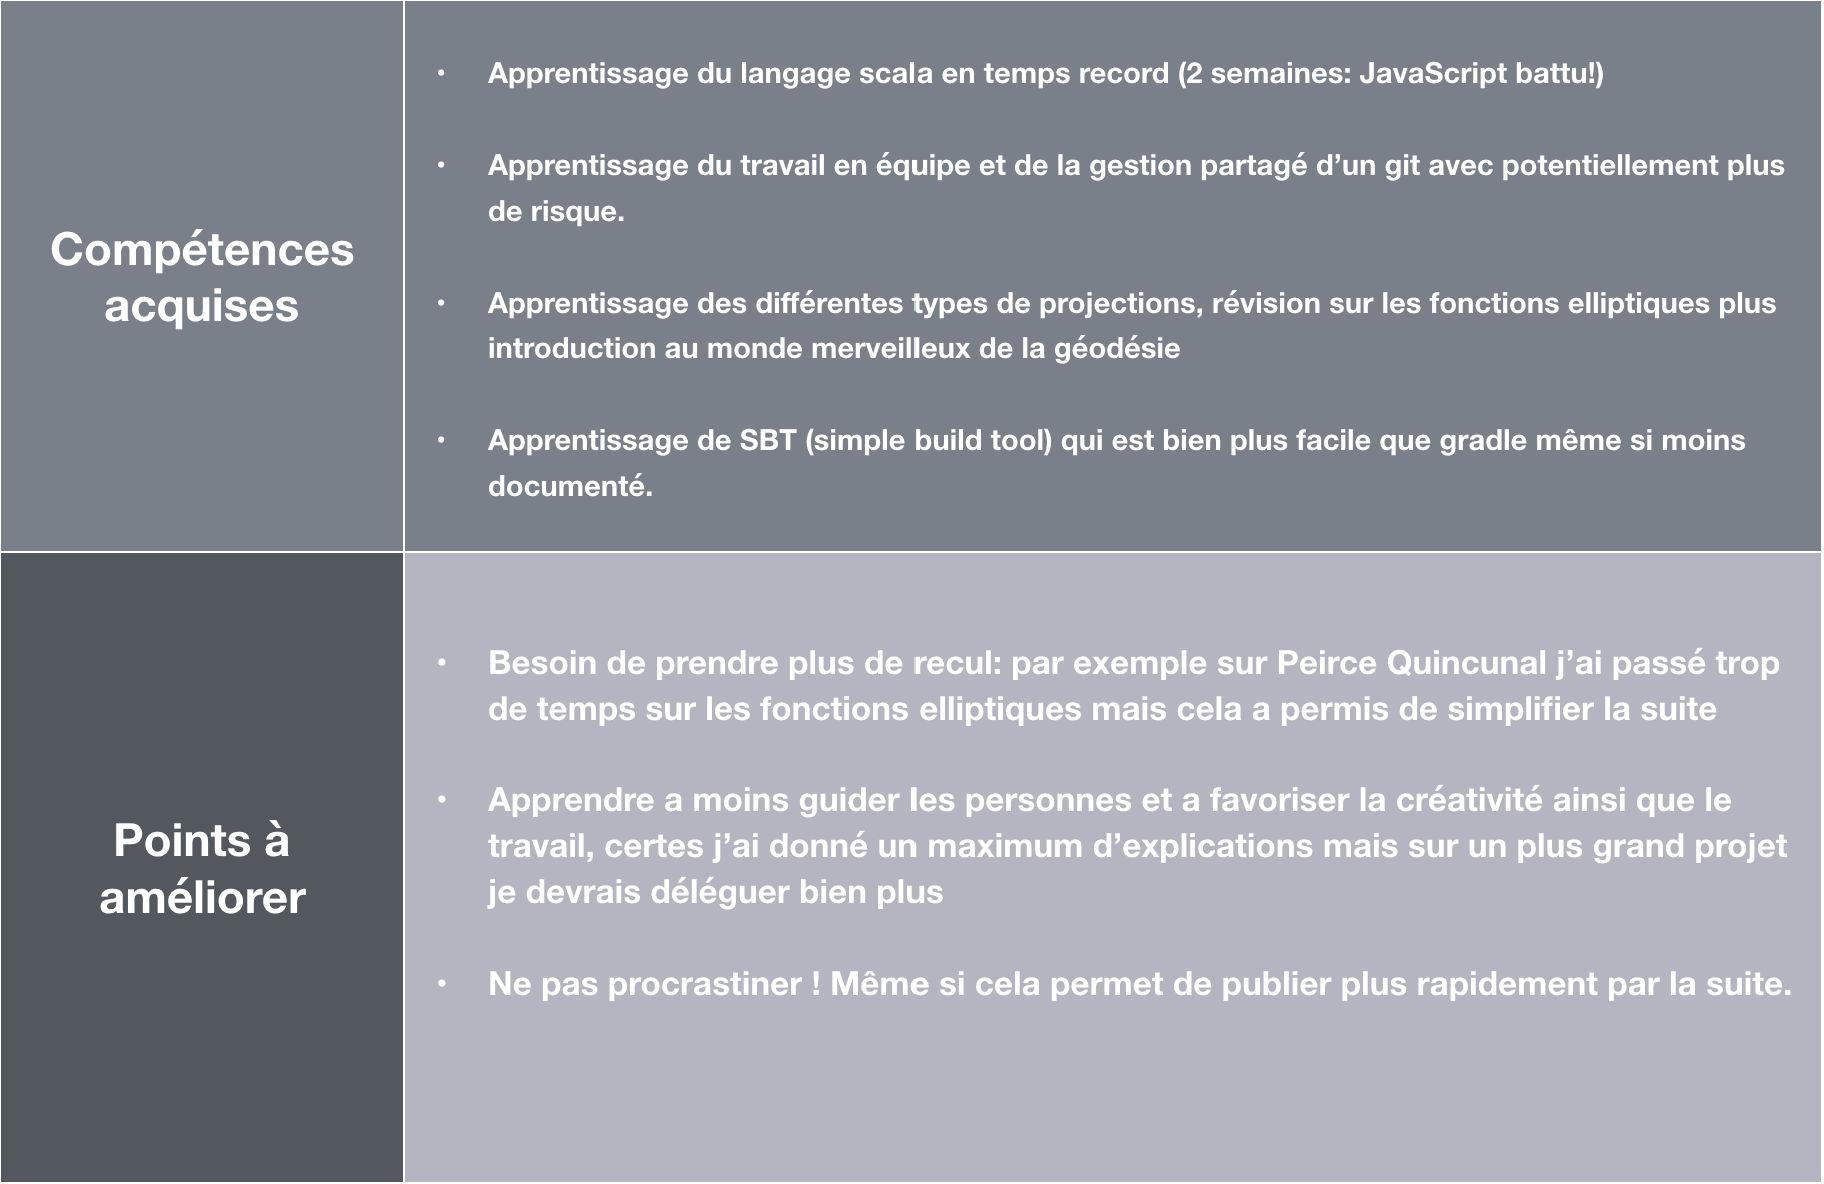
\includegraphics[scale=0.45]{ErwanPM.png}
        \caption{ErwanPM}
        \label{fig:erwanpm}
    \end{figure}
    
    

\section{ Remerciements}


\begin{itemize}
    \item Nous souhaitons remercier l’ensemble de l’équipe pédagogique de Telecom Nancy pour nous avoir enseigné les méthodes et outils indispensable à la réalisation de notre projet.
    \item Plus particulièrement Mr DA SILVA (responsable du projet) et Mme HEURTEL ainsi que Rémi BACHELET pour la gestion de projet.
    \item Nous remercions également Telecom Nancy, pour avoir mis à notre disposition les infrastructures et le matériel informatique nécessaires au projet.
    \end{itemize}

\section{ Sources }


\begin{itemize}
    \item \textbf{Sources des projections} [1] : (https://fr.wikipedia.org/wiki/Projection\_cartographique)
    \begin{itemize}
        \item Projections conformes :
        \begin{itemize}
            \item https://en.wikipedia.org/wiki/Mercator\_projection
            \item https://en.wikipedia.org/wiki/Lambert\_conformal\_conic\_projection
            \item https://en.wikipedia.org/wiki/Transverse\_Mercator\_projection
            \item https://en.wikipedia.org/wiki/Stereographic\_projection
            \item https://en.wikipedia.org/wiki/Peirce\_quincuncial\_projection
            \item https://en.wikipedia.org/wiki/Lee\_Conformal\_Projection
            \item https://en.wikipedia.org/wiki/Guyou\_hemisphere-in-a-square\_projection
            \item https://en.wikipedia.org/wiki/Adams\_hemisphere-in-a-square\_projection
        \end{itemize}
        \newpage
        \item Projections équivalentes :
        \begin{itemize}
            \item https://en.wikipedia.org/wiki/Lambert\_cylindrical\_equal-area\_projection
            \item https://en.wikipedia.org/wiki/Behrmann\_projection
            \item https://en.wikipedia.org/wiki/Eckert\_projection
            \item https://en.wikipedia.org/wiki/Gall–Peters\_projection
            \item https://en.wikipedia.org/wiki/Hobo–Dyer\_projection
            \item https://en.wikipedia.org/wiki/Mollweide\_projection
            \item https://en.wikipedia.org/wiki/Sinusoidal\_projection
            \item https://en.wikipedia.org/wiki/Goode\_homolosine\_projection
            \item https://en.wikipedia.org/wiki/Tobler\_hyperelliptical\_projection
            \item https://en.wikipedia.org/wiki/Equal\_Earth\_projection
        \end{itemize}
    \end{itemize}
    \item \textbf{Image Wrapper} [2] : https://github.com/tncytop/top-roaddetection?fbclid=IwAR36FJKJONnHDibsnBvIsHB53R1sOlaTBIlAwqijN0JS7-KgKKlp\_CkiqD8
\end{itemize}

\vspace{1\baselineskip}
\section{ État de l'art}

\textbf{Définition :} \newline

\noindent{Projection cartographique : Représentation
d'une surface modèle (sphère ou ellipsoïde) sur un plan.} \newline
Il en existe plusieurs types. \newline

\textbf{Type de projections :}
\begin{itemize}
    \item \underline{Cylindrique :} \newline
        On projette l'ellipsoïde sur un cylindre qui l'englobe. Celui-ci peut être tangent au grand cercle, ou sécant en deux cercles. Puis on déroule le cylindre pour obtenir la carte.
    \item \underline{Pseudo-cylindrique :} \newline
        In standard presentation, these map the central meridian and parallels as straight lines. 
        Other meridians are curves (or possibly straight from pole to equator), regularly spaced 
        along parallels.
    \item \underline{Conique :} \newline
        On projette l'ellipsoïde sur une surface conique tangente à une ellipse ou sécant en deux ellipses. Puis on déroule le cône pour obtenir la carte.
    \item \underline{Pseudoconique :} \newline
        In standard presentation, pseudoconical projections represent the central meridian as a 
        straight line, other mer
        idians as complex curves, and parallels as circular arcs.
    \item \underline{Azimutale :} \newline
        On projette l'ellipsoïde sur un plan tangent en un point ou sécant en un cercle.
    \item \underline{Pseudo-azimutale :} \newline
        In standard presentation, pseudoazimuthal projections map the equator
        and central 
        meridian to perpendicular, intersecting straight lines. They map parallels to complex 
        curves bowing away from the equator, and meridians to complex curves bowing in toward 
        the central meridian. Listed here after pseudocylindrical as generally 
        similar to them in 
        shape and purpose.
    \item \underline{Stéréographique :} \newline
    		Le point de perspective est placé sur le sphéroïde ou l'ellipsoïde à l'opposé du 
         plan de projection. Le plan de projection, qui sépare les deux hémisphères nord et sud de la sphère,
         est appelé plan équatorial
    \item \underline{Orthographique :} \newline
    		Le point de perspective est à une distance infinie. On perçoit un hémisphère du globe comme si on
    		était situé dans l'espace. Les surfaces et formes sont déformées, mais les distances sont préservées 
    		sur des lignes parallèles.
\end{itemize}

\vspace{1\baselineskip}

D'autres projections sont calculées seulement avec des formules, et ne sont pas basées sur des projections particulières.

\begin{itemize}
    \item \underline{Polyhédrique :} \newline
        Polyhedral maps can be folded up into a polyhedral approximation to the sphere, using 
        particular projection to map each 
        face with low distortion
\end{itemize}

\textbf{Propriétés :}

\begin{itemize}
    \item \underline{Équivalente :} \newline
        Conserve localement les surfaces.
        is constant in all directions from any chosen point.
    \item \underline{Conforme :} \newline
        Conserve localement les angles, donc les formes.
    \item \underline{Aphylactique :} \newline
        On ne conserve plus de métrique , mais on essaie des réduire les distorsions.
    \item \underline{Equidistante :} \newline
		Conserve les distances sur les méridiens.
    \item \underline{Gnomonique :} \newline
		Transforme les grands cercles en lignes droites.
		Le point de perspective est au centre du sphéroïde. La projection gnomonique conserve les orthodromies, puisque tout arc de grand cercle est projeté en un segment.
\end{itemize}

\textbf{Liste de certaines projections :}
\begin{itemize}
    \item Mercartor (Conforme,Cylindrique) Google Maps utilise cette projection.
    \item Peters (Équivalente,Cylindrique)
    \item Robinson (Pseudo-cylindrique, aphylactique)
    \item Mollweide (Pseudo-cylindrique)
    \item Albers (Conique)
    \item Projection conique conforme de Lambert (Conique,Conforme)
    \item Projection azimutale équivalente de Lambert (Azimutale,Équivalente)
\end{itemize}

\noindent{On peut mélanger différentes projections, utiliser des propriétés mathematiques de certaines fonctions comme 
des sinusoïdes ou encore effectuer des découpages dans une projection afin de la rendre la plus fidèle possible.}
\newline
\noindent{Équivalente et conforme s’excluent mutuellement. Les métriques sont la surface, la forme, les angles , la distance, l’échelle
Toute projection doit s’appuyer sur un datum géodesique , pour cela il existe plusieurs ellipsoïdes courants :} \newline

\begin{itemize}
    \item Clarke 1866
    \item Clarke 1880 anglais
    \item Clarke 1880 IGN
    \item Bessel
    \item Airy
    \item Hayford 1909
    \item International 1924
    \item WGS 66
    \item International 1967
    \item WGS 72
    \item IAG - GRS 80
    \item WGS 84
    \item NADS27
    \item NADS83
    \item OSGB36
    \item ETRS89
    \item ED50
    \item GDA94
    \item JGD2011
    \item Tokyo97
    \item KGD2002
    \item TWD67 et TWD97
    \item BJS54
    \item XAS80
    \item GCJ - 02
    \item BD - 09
    \item PZ - 09.11
    \item GTRF
    \item CGCS200
    \item Hong Kong Princpal Datum
    \item ITRF2014
\end{itemize}



\textbf{Librairies existantes permettant d'effectuer des projections cartographiques :}

\begin{itemize} 
	\item C/C++ : https://proj4.org/
	\item Java : https://github.com/OSUCartography/JMapProjLib et https://github.com/orbisgis/cts
	\item JavaScript : https://github.com/d3/d3-geo-projection/ et http://proj4js.org/
	\item Python : https://github.com/jswhit/pyproj, https://github.com/geo-data/python-epsg et https://			github.com/SciTools/cartopy
	\item Go: https://github.com/pebbe/go-proj-4 ethttps://github.com/omniscale/go-proj
	\item Rust : https://github.com/georust/rust-proj
https://gist.github.com/mbostock/29cddc0006f8b98eff12e60dd08f59a7/raw/373b59870a3cc451ec62c4998082079cf27eb21e/all.gif
\end{itemize}



\end{document}
